\section{Introducción}
En el ámbito universitario resulta necesario mantener informadas a las personas sobre una amplia variedad de hechos, noticias y acontecimientos que sucedieron o sucederán, desde la ubicación de un aula hasta la notificación de la cancelación de una clase. Muchas veces estas notificaciones son sobre cuestiones muy efímeras, lo que requiere rapidez para empezar a transmitirlas y facilidad para tener el alcance necesario.

En las facultades de la Universidad Nacional de La Plata se consumen muchos recursos para cumplir este fin, a través de afiches, pancartas, panfletos, etc. los cuales, pese a ser de barata fabricación, no tienen una vida útil muy extensa. Además todas estas formas de comunicación se basan en el uso de papel, que tras ser utilizado debe desecharse debido a la imposibilidad de reutilizarlo, generando una cantidad de residuos significativa. Si se tiene en cuenta que también generan una polución visual considerable, por la gran cantidad de estos distribuidos en todos los lugares transitables, resulta prudente considerar una nueva forma de comunicación.

% TODO: Mencionar sobre otros carteles comercialmente disponibles
Existen en el mercado varios carteles electrónicos capaces de visualizar mensajes simples, con la particularidad de que suelen requerir que el mensaje sea cambiado manualmente accediendo fisicamente al cartel, lo cual resulta arriesgado al tener en cuenta que este cartel estará en espacios concurridos por cientos de personas.

Surge así la idea de desarrollar de un cartel electrónico, capaz de ser configurado de forma remota y unicamente por las autoridades competentes, con el fin de proveer una forma de comunicación masiva más limpia, clara y menos dañina para el medio ambiente.

En este informe se describe todas las fases del desarrollo de un proyecto para la asignatura Taller de Proyecto 1. El proyecto consiste en el diseño y desarrollo de un sistema de cartel luminoso cuyo contenido es configurable de forma remota. El cartel tiene conectividad WiFi, con lo que es capaz de formar parte de una red IP.

El proyecto utilizó un proceso de desarrollo de cascada, como se muestra en la figura \ref{fig:waterfall}.

\begin{figure}[!ht]
	\centering
	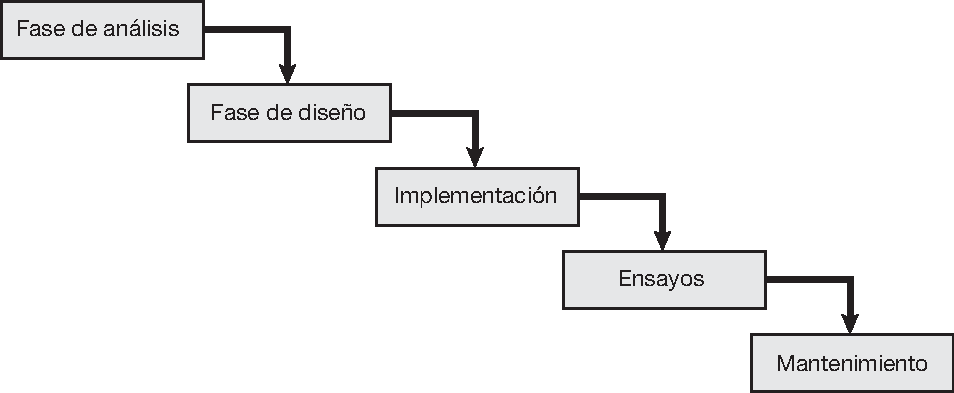
\includegraphics[width=0.8\linewidth]{imagenes/waterfall.pdf}
	\caption{Modelo en cascada de desarrollo.}
	\label{fig:waterfall}
\end{figure}

A lo largo de este informe se documentarán las fases de desarrollo previamente mencionadas.

En la sección \ref{part:analisis} se habla sobre los requerimientos y especificaciones del sistema, detallando que funcionalidades debe tener y a cuáles restricciones está sujeto.

Luego, en la sección \ref{part:diseno}, se mencionan las componentes que constituyen el sistema, se explicitan modelos que describen el comportamiento del sistema, la interfaz de usuario y la arquitectura del software. También se muestran los esquemáticos que especifican la conexión de los componentes.

En la sección de implementación se documenta como se fue dando el proceso de desarrollo de software y la implementación física del hardware.

En la sección de ensayos se documenta los resultados de las pruebas que se realizaron sobre el sistema en funcionamiento.

Por último, se anexa como apéndice un detalle del presupuesto requerido para la realización del proyecto, más una guía instructiva que explica los pasos necesarios para poner en marcha el sistema, junto a más piezas de información que el equipo considera de interés para el entendimiento pleno del proyecto y de su implementación.

\section{Objetivos del proyecto}
El objetivo primario de este proyecto es el diseño e implementación de un cartel luminoso que pueda ser configurado remotamente por un usuario. No se tiene como objetivo realizar un producto diseñado de manera que sea económicamente viable producirlo en masa, sino más bien el desarrollo de un prototipo a modo de prueba de concepto. El sistema a desarrollar deberá responder a varias necesidades de operabilidad, conectividad y funcionamiento.

El objetivo puede ser divido en los siguientes subobjetivos:
\begin{itemize}
	\item Diseño general de la solución.
	\item Diseño e implementación del hardware que controla el cartel.
	\item Diseño e implementación del software mediante el cual se establece el contenido del cartel de forma remota.
	\item Diseño e implementación del protocolo de comunicación por el cual interactuarán las componentes.
\end{itemize}

En la parte \ref{part:analisis} se explicitará las funcionalidades que debe tener el sistema y la interfaz de usuario que expone.
